\documentclass[11pt]{article}

\usepackage[T1]{fontenc}
\usepackage[margin=1in]{geometry}
\usepackage{amsmath,amssymb,mathtools,bm}
\usepackage{booktabs,longtable,array,multirow}
\usepackage{graphicx}
\usepackage{xcolor}
\usepackage{xurl}
\usepackage{hyperref}
\hypersetup{hidelinks}
\urlstyle{tt}

\newcommand{\R}{\mathbb{R}}
\newcommand{\dd}{\,\mathrm{d}}
\newcommand{\E}{\mathbb{E}}
\newcommand{\KL}{D_{\mathrm{KL}}}
\newcommand{\ESS}{\mathrm{ESS}}
\newcommand{\IAT}{\tau_{\mathrm{int}}}
\newcommand{\Rhat}{\widehat R}
\newcommand{\one}{\mathbf{1}}
\newcommand{\piB}{\pi_\beta}
\newcolumntype{L}[1]{>{\raggedright\arraybackslash}p{#1}}
\setlength{\emergencystretch}{3em}

\title{Numerical Experiments for L\'evy Score-Corrected\\
Compound-Poisson Equilibrium Sampling}
\author{}
\date{}

\begin{document}
\maketitle

\begin{abstract}
We evaluate L\'evy score-corrected compound-Poisson (LSC-CP) sampling on four
multimodal Boltzmann model systems: a one-dimensional double well, a planar
forty-mode Gaussian mixture, a depth-balanced three-well M\"uller--Brown
landscape embedded in ten dimensions, and a coupled $\phi^4$ chain in
twenty-four dimensions.  Across the reported horizons, LSC-CP markedly reduces
terminal basin-population error relative to local samplers and raw
compound-Poisson dynamics, and it yields nonzero post-settling effective
sample sizes for every basin indicator.  The MoG40 global $W_2$ and MMD
discrepancies remain above their finite-sample reference bands, so the results
do not imply that every distributional metric reaches its sampling floor.
The implementation uses finite chord quadrature, tamed Euler updates, an
exponent cap, and projection onto a finite computational box.  These practical
stabilizations control overflow and large updates and improve numerical
robustness in the stiff score regime, but they define an approximate
finite-step kernel.  Statistically resolved
potential-energy biases are therefore reported explicitly.  The evidence
supports accelerated interbasin exploration and accurate population recovery
with observable-dependent numerical bias, rather than exact finite-step
Boltzmann sampling.  No physical kinetics is inferred.
\end{abstract}

\section{Overview and compared methods}
\label{sec:overview}

All experiments target a Boltzmann law
\begin{equation}
 \piB(x)=Z_\beta^{-1}e^{-\beta V(x)},\qquad x\in\R^d .
 \label{eq:target}
\end{equation}
The sampler of interest augments overdamped Langevin dynamics with a finite
compound-Poisson jump process of measure $\nu(\dd r)=\lambda\rho(\dd r)$ and
adds the stationary L\'evy-score drift $S_{\nu,\beta}$ so that the combined
generator
\begin{equation}
 A_{\nu,\beta}f
 =\bigl[-\nabla V+S_{\nu,\beta}\bigr]\cdot\nabla f
  +\beta^{-1}\Delta f+J_\nu f
 \label{eq:corrected-generator}
\end{equation}
is weakly stationary for $\piB$ (Appendix~\ref{app:construction}).  The
practical estimators evaluate the score integral by deterministic chord
quadrature where affordable and by \emph{paired} random-bank estimators in
higher dimension: the realized jump displacements and the L\'evy-score drift of
one step are generated from the same random finite measure.  This pairing
aligns the drift and jump measures before the remaining finite chord
quadrature is applied (Appendix~\ref{app:paired}).  Figures label the
implemented estimator simply \textsc{lsc-cp}.  The reported variants are:
deterministic shell quadrature (double well), a semi-analytic score with
angular quadrature (MoG40), the paired
single-atom estimator \textsc{lsc-cp-ra} (double
well and MoG40, as an estimator-agreement check), and the paired multi-atom
estimator \textsc{lsc-cp-ma} (M\"uller--Brown and $\phi^4$).

Baselines are the unadjusted Langevin algorithm (\textsc{ula}), Metropolis
adjusted Langevin (\textsc{mala}), the BAOAB underdamped integrator
(\textsc{baoab}), an $\alpha$-stable L\'evy-flight analogue (\textsc{fla}),
and parallel tempering (\textsc{pt}) with an automatically tuned ladder and
fully counted replica cost.  Raw compound Poisson (\textsc{cp}), i.e.\ the
same jump bank \emph{without} the score correction, is included as a
stationarity-defect ablation: its invariant law is not $\piB$, so it is a
control for the value of the correction, not a fair efficiency baseline.  All
methods share per-seed initial ensembles.  In the double-well and MoG40
full-law experiments, \textsc{cp} and deterministic/closed-form
\textsc{lsc-cp} additionally share the jump random stream pathwise.  In the
M\"uller--Brown and $\phi^4$ experiments, raw full-law \textsc{cp} and
\textsc{lsc-cp-ma} match the marginal jump geometry, weights, and intensity,
but do not use the same realized random banks and hence are not pathwise
paired.

The implemented scheme uses finite chord quadrature, log-domain accumulation
with an exponent cap, tamed Euler drift updates, and projection onto a finite
computational domain to stabilize evaluation in the stiff-score regime.  These
operations define the finite-step algorithm evaluated below.  The stationarity
identity applies to the ideal continuous-time generator with the exact,
uncapped L\'evy-score field on an unbounded state space.  We assess the
equilibrium fidelity of the discretization through timestep and quadrature
sensitivity checks, observable biases, and cap/projection activation rates.
Passage statistics are interpreted solely as algorithmic mixing diagnostics;
no physical reaction kinetics is inferred.

\section{Benchmark systems}
\label{sec:systems}

\begin{table}[ht]
\centering
\small
\setlength{\tabcolsep}{5pt}
\begin{tabular}{lllll}
\toprule
 & Double well & MoG40 & Depth-balanced MB & Coupled $\phi^4$\\
\midrule
dimension $d$        & 1 & 2 & 10 & 24\\
$\beta$              & 8 & 8 & 24 & 8\\
particles $N$        & 16{,}000 & 2{,}500 & 2{,}000 & 1{,}000\\
horizon $T$          & 100 & 100 & 200 & 100\\
$\Delta t$ (used)    & 0.005 & 0.010 & 0.005 & 0.002\\
steps                & 20{,}000 & 10{,}000 & 40{,}000 & 50{,}000\\
seeds                & 24 & 24 & 16 & 16\\
jump rate $\lambda$  & 1 & 1 & 1 & 1\\
score quadrature     & $q_\theta{=}16$, $q_\rho{=}4$ & analytic $\theta,\rho$; $m_\phi{=}16$ & $q_\theta{=}8$, $q_\rho{=}4$ & $q_\theta{=}32$, $q_\rho{=}4$\\
score estimator      & deterministic + \textsc{ra} & semi-analytic + \textsc{ra} & \textsc{ma} & \textsc{ma}\\
weak-identity residual & $1.5\times10^{-7}$ & $3.0\times10^{-8}$ & $5.0\times10^{-7}$ & $2.0\times10^{-7}$\\
\bottomrule
\end{tabular}
\caption{Reported numerical configurations and uncapped weak drift--jump
identity residuals (diagnostic tolerance $10^{-6}$;
Appendix~\ref{app:stability}).  The residual measures generator-level
drift--jump cancellation for a finite family of test functions.  Full model,
bank, and ladder specifications are
in Appendix~\ref{app:specs}.}
\label{tab:configs}
\end{table}

\paragraph{Double well ($d=1$).}
$V(x)=(x^2-1)^2$ at $\beta=8$: two equal wells at $\pm1$ separated by a
dimensionless barrier $\beta\Delta V=8$.  The jump bank is a symmetric shell
at $\pm2$ with radial half-width $0.2$.  This is the transparent two-state
test of target recovery and interwell communication.

\paragraph{MoG40 ($d=2$).}
$\piB$ is an equal-weight mixture of forty unit-covariance Gaussians;
$V(x)=-\beta^{-1}\log\sum_{k}\exp[-\lVert x-\mu_k\rVert^2/2]$.  The jump law
is deliberately generic: radius uniform on $[4,15]$ (set from the
nearest-neighbour distance histogram alone), direction uniform on the circle.
Neither \textsc{pt} nor \textsc{lsc-cp} receives the mode locations.  This is
the many-basin stress test.

\paragraph{Depth-balanced M\"uller--Brown ($d=10$).}
A M\"uller--Brown-type three-well landscape whose well depths are retuned to
be equal, evaluated in a two-dimensional latent plane and embedded in ten
dimensions by a fixed linear map with Gaussian auxiliary coordinates
($\sigma_{\rm aux}=0.4$), at $\beta=24$.  The equal depths separate
multimodality from metastability: the channels retain dimensionless barriers
$\beta b_{AB}\simeq11.1$ and $\beta b_{BC}\simeq4.0$ while the equilibrium
masses stay comparable.  The bank has four directed relay atoms
$A\leftrightarrow B\leftrightarrow C$ (no direct $A$--$C$ atom), so transport
must use the relay through $B$.  This tests curved, nonuniform basins and a
designed jump graph.

\paragraph{Coupled $\phi^4$ chain ($d=24$).}
Twelve periodic two-component sites,
$V(q)=\tfrac{\kappa}{2\delta}\sum_i\lVert q_{i+1}-q_i\rVert^2
+\delta\sum_iW(q_i)$ with $\kappa=2.5$, $\delta=1/12$, $\beta=8$, and a tilted
double-double-well site potential $W$ (Appendix~\ref{app:specs}).  The target
has four coherent phases; the bank has eight directed edge atoms along the
phase square (diagonals excluded because their coherent chords cross the
field-zero hilltop).  The primary collective variable is the spatial mean
$\bar q=\tfrac1{12}\sum_iq_i\in\R^2$.  This is the many-body example: a
collective transition in a coupled field.

The four systems form a hierarchy of equilibrium questions---two-state
balance, many-mode occupancy, curved-basin relay transport, and a collective
field transition---rather than four independent leaderboard tasks.

\section{Protocol, references, and numerical parameter selection}
\label{sec:protocol}

\paragraph{Run protocol.}
For each system all seeds are batched into one ensemble per method with
per-seed initial blocks; every method starts from the identical localized
per-seed ensemble.  We used dyadic timestep sensitivity checks based on
terminal $W_2$, basin TV, MMD, and energy-moment-consistency diagnostics for
the $\piB$-targeting methods.  The non-targeting \textsc{fla} and raw
\textsc{cp} chains were recorded but did not determine the timestep.  Score
quadrature was selected analogously, with the additional uncapped
weak-identity residual.  These checks guided numerical parameter selection,
but they did not include post-settling mean energy or collective-variable bias
and therefore do not establish convergence of the invariant measure of the
stabilized chain.

\paragraph{References and floors.}
The double well uses a dense-grid inverse-CDF reference; MoG40 an exact
mixture draw; M\"uller--Brown a fine two-dimensional latent grid combined
with exact Gaussian auxiliaries; $\phi^4$ a Laplace-mixture proposal corrected
by self-normalized importance weights (direct SNIS for basin masses, energy
moments, CV means, and the free-energy surface; finite
sampling-importance-resampling only where unweighted clouds are required).
The $\phi^4$ weight diagnostics for the reference are: $2\times
10^5$ proposals, weight ESS $41{,}182$ (fraction $0.206$), maximum normalized
weight $3.6\times10^{-3}$ (Appendix~\ref{app:references}).  A separate
$t=300$ parallel-tempering check gave phase masses
$(0.365,0.204,0.234,0.197)$, whose TV distance from the SNIS masses is
$0.042$.  Consequently, differences below this scale in the $\phi^4$ basin
metrics are reference sensitive.  For every metric, a finite-sample
\emph{floor} is estimated by comparing two independent
reference draws of the same size; ``at the floor'' below means within the
floor band $\text{mean}+3\,\text{sd}$.

\paragraph{Stability diagnostics.}
We monitored nonfinite states, score-cap and state-box projection frequencies,
jump-boundary contact per applied jump, and basin-map-domain escape.  The
uncapped weak-identity residual was evaluated on a domain extending at least
one maximum jump beyond the high-probability region.  The measured values and
domain-coverage rationale appear in Appendix~\ref{app:stability}.  These
quantities diagnose numerical robustness and exposure to the stabilizations;
small activation frequencies do not prove that the finite-step kernel has
invariant law $\piB$.

\section{Equilibrium recovery}
\label{sec:recovery}

\begin{table}[p]
\centering
\footnotesize
\setlength{\tabcolsep}{3pt}
\begin{tabular}{llllll}
\toprule
Method & $W_2$ & $\mathrm{TV}_{\rm basin}$ & $\mathrm{RMSE}_{F}/k_{\rm B}T$
 & $\KL(p^\star\Vert\widetilde p)$ & FES outside\\
\midrule
\multicolumn{6}{l}{\emph{Double well} \hfill (floors: $W_2$ $0.061\pm0.033$, TV $0.0032\pm0.0017$)}\\
\textsc{ula}   & 1.26 (0.003) & 0.471 (0.001) & 1.77 (0.02) & 1.09 (0.02) & 0\\
\textsc{mala}  & 1.26 (0.003) & 0.473 (0.001) & 1.79 (0.02) & 1.12 (0.02) & 0\\
\textsc{baoab} & 1.29 (0.002) & 0.488 (0.001) & 2.23 (0.04) & 1.54 (0.04) & 0\\
\textsc{fla}   & 0.096 (0.018) & 0.0033 (0.003) & 0.302 (0.008) & $3.4\times10^{-5}$ & 0.003\\
\textsc{pt}    & 0.064 (0.032) & 0.0033 (0.002) & 0.050 (0.009) & $3.2\times10^{-5}$ & 0\\
\textsc{cp}    & 0.176 (0.013) & 0.0036 (0.003) & 0.157 (0.006) & $4.2\times10^{-5}$ & 0.029\\
\textsc{lsc-cp}    & 0.111 (0.017) & 0.0036 (0.003) & 0.168 (0.009) & $4.4\times10^{-5}$ & 0.005\\
\textsc{lsc-cp-ra} & 0.131 (0.017) & 0.0031 (0.003) & 0.180 (0.010) & $3.2\times10^{-5}$ & 0.008\\
\midrule
\multicolumn{6}{l}{\emph{MoG40} \hfill (floors: $W_2$ $1.31\pm0.28$, TV $0.051\pm0.006$)}\\
\textsc{ula}   & 26.1 (0.02) & 0.916 (0.003) & 1.81 (0.01) & 4.20 (0.02) & 0\\
\textsc{mala}  & 26.1 (0.03) & 0.917 (0.003) & 1.81 (0.01) & 4.21 (0.01) & 0\\
\textsc{baoab} & 26.2 (0.03) & 0.930 (0.005) & 1.77 (0.01) & 4.24 (0.02) & 0\\
\textsc{fla}   & 15.2 (0.21) & 0.436 (0.007) & 1.37 (0.06) & 0.743 (0.05) & 0.001\\
\textsc{pt}    & 6.54 (0.34) & 0.141 (0.007) & 0.350 (0.02) & 0.055 (0.005) & 0\\
\textsc{cp}    & 9.98 (0.19) & 0.286 (0.009) & 0.680 (0.04) & 0.267 (0.013) & 0.254\\
\textsc{lsc-cp}    & 2.83 (0.34) & 0.064 (0.008) & 0.190 (0.02) & 0.012 (0.003) & 0.001\\
\textsc{lsc-cp-ra} & 2.65 (0.26) & 0.103 (0.009) & 0.280 (0.02) & 0.036 (0.006) & 0.005\\
\midrule
\multicolumn{6}{l}{\emph{Depth-balanced MB, 10D} \hfill (floors: $W_2$ $0.050\pm0.020$, TV $0.011\pm0.007$)}\\
\textsc{ula}   & 0.409 (0.003) & 0.307 (0.002) & 2.27 (0.23) & 1.17 (0.14) & 0\\
\textsc{mala}  & 0.411 (0.003) & 0.308 (0.001) & 2.32 (0.18) & 1.22 (0.16) & 0\\
\textsc{baoab} & 0.415 (0.003) & 0.309 (0.001) & 2.50 (0.17) & 1.52 (0.21) & 0\\
\textsc{fla}   & 0.179 (0.006) & 0.119 (0.008) & 0.941 (0.04) & 0.048 (0.007) & 0.039\\
\textsc{pt}    & 0.056 (0.021) & 0.013 (0.008) & 0.132 (0.02) & $5.7\times10^{-4}$ & 0\\
\textsc{cp}    & 0.353 (0.008) & 0.135 (0.006) & 0.267 (0.02) & 0.047 (0.005) & 0.172\\
\textsc{lsc-cp-ma} & 0.047 (0.009) & 0.014 (0.006) & 0.136 (0.010) & $5.8\times10^{-4}$ & 0.006\\
\midrule
\multicolumn{6}{l}{\emph{Coupled $\phi^4$, 24D} \hfill (floors: $W_2$ $0.130\pm0.035$, TV $0.024\pm0.010$)}\\
\textsc{ula}   & 1.22 (0.004) & 0.671 (0.003) & 2.59 (0.09) & 3.07 (0.31) & 0\\
\textsc{mala}  & 1.22 (0.004) & 0.673 (0.002) & 2.63 (0.05) & 3.13 (0.17) & 0\\
\textsc{baoab} & 1.22 (0.006) & 0.673 (0.002) & 2.64 (0.05) & 3.14 (0.22) & 0\\
\textsc{fla}   & 0.194 (0.032) & 0.060 (0.013) & 0.220 (0.03) & 0.011 (0.004) & $10^{-4}$\\
\textsc{pt}    & 0.364 (0.028) & 0.119 (0.015) & 0.315 (0.04) & 0.039 (0.008) & 0\\
\textsc{cp}    & 0.410 (0.021) & 0.077 (0.016) & 0.482 (0.05) & 0.017 (0.006) & 0.209\\
\textsc{lsc-cp-ma} & 0.100 (0.028) & 0.022 (0.011) & 0.151 (0.03) & 0.0015 (0.001) & 0.003\\
\bottomrule
\end{tabular}
\caption{Terminal metrics at $t=T$, mean (std) over seeds.  $W_2$: sliced
(exact in 1D) Wasserstein-2 against the reference in metric space;
$\mathrm{TV}_{\rm basin}$: total variation of basin occupancy;
$\mathrm{RMSE}_F$: additive-aligned free-energy-surface RMSE in $k_{\rm B}T$
on the two-dimensional collective variables (one-dimensional for the double
well); $\KL$: target-to-empirical basin KL with Jeffreys pseudocount; FES
outside: empirical mass outside the frozen reference FES grid.  Metric
definitions in Appendix~\ref{app:metrics}.}
\label{tab:terminal}
\end{table}

\begin{figure}[ht]
\centering
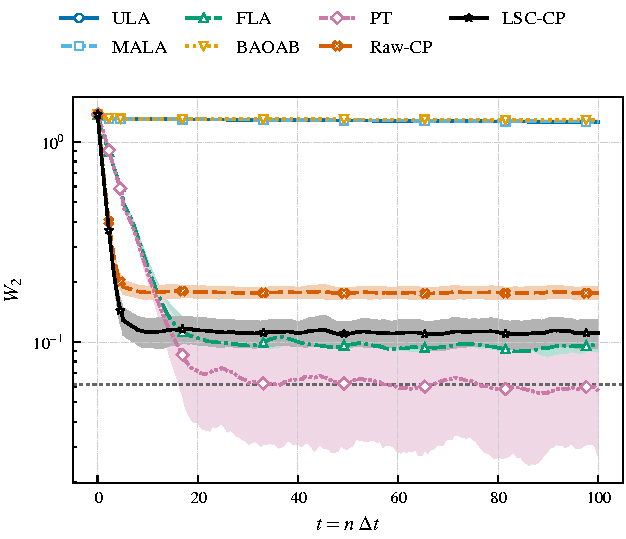
\includegraphics[width=0.49\textwidth]{figs/double_well_W2_t.pdf}
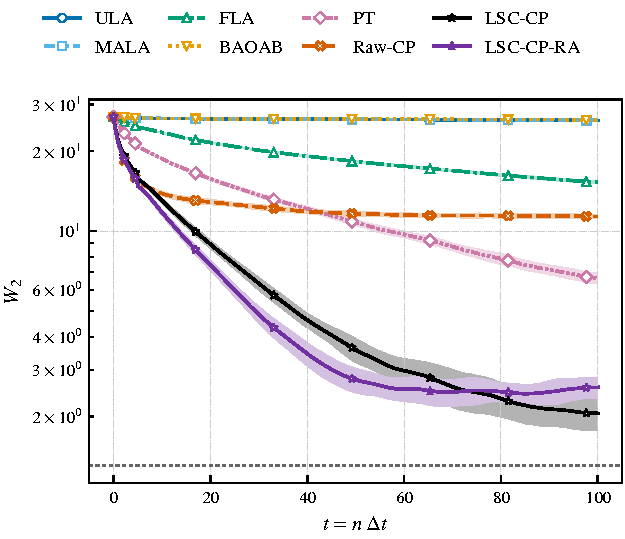
\includegraphics[width=0.49\textwidth]{figs/mog40_W2_t.pdf}\\[2pt]
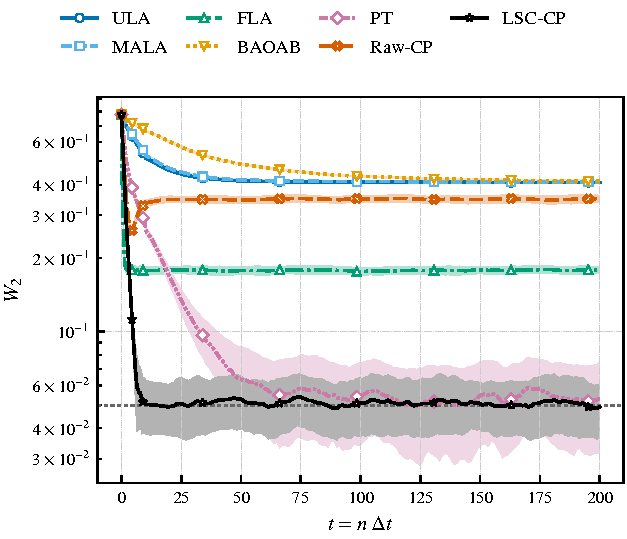
\includegraphics[width=0.49\textwidth]{figs/mb3well_10d_W2_t.pdf}
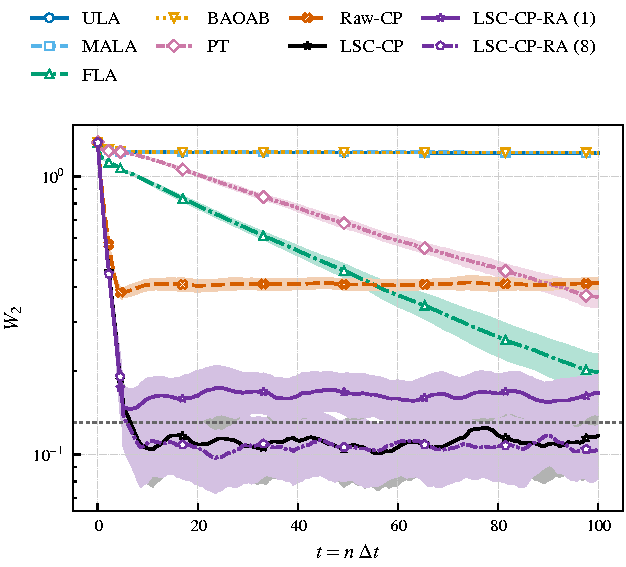
\includegraphics[width=0.49\textwidth]{figs/coupled_phi4_W2_t.pdf}
\caption{Ensemble relaxation: $W_2$ to the reference versus simulation time
$t$ from the shared localized initial ensembles (seed-band envelopes).
Top: double well, MoG40; bottom: M\"uller--Brown 10D, coupled $\phi^4$.}
\label{fig:relaxation}
\end{figure}

Four observations organize Table~\ref{tab:terminal} and
Figure~\ref{fig:relaxation}.

\emph{(i) Local dynamics remain strongly metastable.}
On every system, the terminal \textsc{ula}, \textsc{mala}, and \textsc{baoab}
ensembles remain strongly localized relative to the target (basin TV
$0.31$--$0.93$, basin KL $1.1$--$4.2$).  Occasional label changes occur in
some of the post-settling MoG40 and M\"uller--Brown traces, but they are too
sparse to recover all basin populations.  This quantifies the metastability
that the nonlocal methods are intended to address.

\emph{(ii) LSC-CP improves basin recovery, with metric-dependent residual
error.}
The reported LSC-CP estimator attains basin TV and KL at or within the
finite-sample floor band on the double well, M\"uller--Brown, and $\phi^4$;
the last comparison is subject to the independent-reference uncertainty noted
in Section~\ref{sec:protocol}.  Its MoG40 basin TV, $0.064$, is also within the
upper reference band, $0.051+3(0.006)=0.069$.  The corresponding global
$W_2=2.83$ exceeds its upper reference band of approximately $2.15$, however,
and MMD $=0.0482$ exceeds its upper band of approximately $0.0317$.  On MoG40,
the raw-jump and \textsc{pt} basin-TV errors are respectively $4.5$ and
$2.2$ times the LSC-CP value, while \textsc{lsc-cp-ra} is $1.6$ times larger.
Parallel tempering matches LSC-CP on the double well and M\"uller--Brown but
has larger basin KL on MoG40 ($0.055$ versus $0.012$) and $\phi^4$ ($0.039$
versus $0.0015$) at full replica cost.  The latter distinction is
reference-sensitive below the $0.042$ scale.  The $\alpha$-stable flight is
competitive on the double well but shows much larger discrepancies elsewhere
(e.g., MB free-energy RMSE $0.94\,k_{\rm B}T$).

\emph{(iii) The score correction substantially reduces the raw-jump
distortion.}
In the double-well and MoG40 full-law runs, raw \textsc{cp} and
\textsc{lsc-cp} share jump streams pathwise.  The MB and $\phi^4$ comparisons
instead match the marginal bank geometry, weights, and intensity but are not
pathwise paired.  Raw \textsc{cp} retains basin TV $0.286/0.135/0.077$ on
MoG40/MB/$\phi^4$, and $17$--$25\%$ of its terminal mass lies outside the
reference free-energy grid on the three multivariate systems, versus
$\le0.6\%$ for LSC-CP.  Raw \textsc{cp} also contacts the finite box on
$2.5\%$, $6.7\%$, and $0.4\%$ of applied jumps on these systems
(Appendix~\ref{app:stability}); this is a numerical-box confound, especially
for MoG40 and MB, rather than an intrinsic component of the stationary
defect.  In one $\phi^4$ sensitivity comparison, widening the box from
$[-2,2]^{24}$ to $[-5,5]^{24}$ changes raw-CP $W_2$ from $0.28$ to $0.41$,
whereas LSC-CP-\textsc{ma} changes from $0.099$ to $0.100$.  This single check
supports robustness to that particular box change but does not establish
general box-size independence.

\emph{(iv) Random-bank and deterministic estimators are qualitatively
consistent.}
Where both are run (double well and MoG40), the paired single-atom estimator
preserves the qualitative method ordering and gives comparable terminal
errors on several metrics.  It is not numerically equivalent on every metric:
for example, the MoG40 basin KL is $0.036$ versus $0.012$ (a factor of about
three), and the outside-grid mass is about four times larger.  The comparison
therefore provides an estimator-sensitivity check, not a proof of equivalence
or a validation of the multi-atom approximation.

\section{Post-settling time-series diagnostics}
\label{sec:efficiency}

Terminal ensemble metrics quantify the law at time $T$; they do not measure
the precision of time averages.  For that purpose, small independent chains
(4 seeds $\times$ 8 chains, 1000 uniformly spaced draws over one additional
horizon) are initialized from the system reference, evolved for one full
settling horizon, and then analyzed for basin indicators, energy, and
collective variables.  None is claimed to be an exact stationary draw of the
discrete kernel, so the values below are post-settling diagnostics of the
numerical chains (Appendix~\ref{app:metrics}).  A constant basin indicator
contributes zero ESS by construction.  Raw \textsc{cp} and \textsc{fla} are
excluded because their invariant laws are not $\piB$.

\begin{table}[!ht]
\centering
\footnotesize
\setlength{\tabcolsep}{2.5pt}
\begin{tabular}{lrrrr|rrrr}
\toprule
 & \multicolumn{4}{c|}{worst-basin ESS (of 32{,}000)} &
   \multicolumn{4}{c}{energy ESS / signed energy bias}\\
Method & DW & MoG40 & MB & $\phi^4$ & DW & MoG40 & MB & $\phi^4$\\
\midrule
\textsc{ula}   & 0 & 0 & 0 & 0 & 14{,}815 / $+0.0003$ & 707 / $+0.001$ & 22{,}223 / $+0.007$ & 17{,}212 / $+0.133$\\
\textsc{mala}  & 0 & 0 & 0 & 0 & 14{,}869 / $+0.0005$ & 710 / $-0.004$ & 21{,}994 / $-0.001$ & 15{,}250 / $-0.010$\\
\textsc{baoab} & 0 & 0 & 0 & 0 & 3{,}658 / $-0.0002$ & 534 / $-0.001$ & 5{,}622 / $+0.004$ & 2{,}734 / $+0.028$\\
\textsc{pt}    & 1{,}211 & 572 & 2{,}336 & 2{,}567 & 20{,}494 / $-0.001$ & 1{,}340 / $+0.0006$ & 25{,}202 / $-0.0004$ & 24{,}383 / $-0.002$\\
\textsc{lsc-cp}$^{(\ast)}$ & 1{,}648 & 229 & 1{,}952 & 1{,}150 & 31{,}891 / $+0.194$ & 22{,}718 / $+0.114$ & 26{,}720 / $+0.039$ & 30{,}972 / $+0.251$\\
\textsc{lsc-cp-ra} & 1{,}809 & 59 & --- & --- & 31{,}224 / $+0.247$ & 9{,}165 / $+0.448$ & --- & ---\\
\bottomrule
\end{tabular}
\caption{Post-settling trace diagnostics aggregated over all seeds and chains.
Worst-basin ESS is the minimum, over basins, of the summed per-chain effective
sample size of that basin's indicator (Geyer IAT; constant chains contribute
zero).  Energy bias is the signed difference between the trace mean of $V$ and
the reference target, in energy units; it is interpreted with its
observable-specific Monte Carlo standard error.  $^{(\ast)}$\textsc{lsc-cp}
row: deterministic/semi-analytic score on DW and MoG40, paired multi-atom on
MB and $\phi^4$.  Split-$\Rhat$ and MCSE values for every observable are
reported in the supporting data.}
\label{tab:ess}
\end{table}

The LSC energy MCSEs are $0.0194$ (double well), $0.00485$ (MoG40),
$0.00143$ (MB), and $0.0141$ ($\phi^4$); the corresponding double-well and
MoG40 random-atom values are $0.0273$ and $0.0164$.  Energy split-$\Rhat$ is
below $1.11$ for the tabulated methods, but this does not extend to every
basin or collective-variable trace.  For example, maximum values are $1.70$
for MoG40 LSC-CP, $1.61$ for MoG40 LSC-CP-RA, $1.28$ for MoG40 PT, and $1.13$
for $\phi^4$ PT.  We therefore use these quantities as finite-horizon
diagnostics and interpret them jointly with population errors.

Three conclusions follow from Table~\ref{tab:ess}.

\emph{(i) Between-basin ESS separates the methods qualitatively.}
The three local integrators record \emph{exactly zero} worst-basin ESS on
every system because at least one basin indicator is constant or unvisited in
the recorded traces.  This is not equivalent to zero transitions: on MoG40,
for example, \textsc{ula}, \textsc{mala}, and \textsc{baoab} record 222, 230,
and 60 label changes, and the corresponding MB counts are 209, 194, and 43.
Their large energy ESS values illustrate why energy decorrelation alone is
insufficient evidence of global mixing.  LSC-CP sustains worst-basin ESS
between $229$ and $1{,}952$---the same order as fully costed parallel
tempering---using local gradients and the jump-bank score.

\emph{(ii) Mixing and accuracy must be read together.}
On MoG40 and $\phi^4$, \textsc{pt} has the larger post-settling worst-basin
ESS ($572$ versus $229$; $2{,}567$ versus $1{,}150$), whereas LSC-CP has
smaller terminal basin KL at the reported horizon (Table~\ref{tab:terminal}).
The $\phi^4$ population difference is reference-sensitive as discussed above.
Neither diagnostic alone ranks the samplers; population error, observable
bias, mixing, and computational cost must be reported together.

\emph{(iii) The LSC chains carry a measurable energy bias.}
The post-settling energy mean of the LSC chains exceeds the target by $+0.04$
to $+0.25$ energy units, and the MCSE values above resolve these differences.
The local methods are not uniformly unbiased either: on $\phi^4$, the signed
biases are $+0.1334$ for \textsc{ula}, $-0.0100$ for \textsc{mala}, and
$+0.0276$ for \textsc{baoab}.  The LSC bias cannot be attributed merely to
high-energy post-jump chord configurations, because those transients also
occur in the exact continuous-time process whose drift--jump balance preserves
$\piB$.  Instead, it indicates observable-dependent invariant-measure error
in the finite-step kernel, potentially from Euler splitting, drift taming,
finite quadrature, exponent capping, or box projection.  These devices are
useful for robust computation, but systematic refinement is needed to
separate their contributions to the measured bias.

\emph{Cost-normalized throughput.}
Per-second comparisons are restricted to MB and $\phi^4$, which were timed on
a dedicated H200 GPU.  On MB, LSC-CP and \textsc{pt} yield respectively
$33.03$ and $48.23$ energy ESS/s, while their worst-basin throughputs are
$2.41$ and $4.47$ ESS/s.  LSC-CP evaluates $Aq_\theta=4\times8=32$
score-quadrature energy differences per particle step.  On $\phi^4$, the
energy throughputs are $50.80$ and $62.17$ ESS/s and the worst-basin
throughputs are $1.89$ and $6.55$ ESS/s, with $Aq_\theta=8\times32=256$ for
LSC-CP.  Per-gradient, per-potential, and per-score-quadrature ESS are included
for every observable in the supporting data; accounting conventions are given
(Appendix~\ref{app:computational}).

\section{Scope and limitations}
\label{sec:outlook}

Three boundaries of the present evidence are stated explicitly.  First, all
results are equilibrium-sampling diagnostics of algorithmic chains; passage
or round-trip statistics, where recorded, are Kaplan--Meier restricted means
of algorithmic mixing times and carry no molecular-kinetics meaning.  Second,
the finite-step LSC chains are not exactly $\piB$-invariant, and the measured
consequences---the energy bias of Section~\ref{sec:efficiency} and the
clipping/boundary diagnostics of Appendix~\ref{app:stability}---are part of
the reported results.  Third, the present comparison does not include a
matched-length \emph{random-geometry} jump control (same atom count, length
multiset, weights, rate, and cost; randomized directions) that would isolate
the contribution of the designed bank geometry from the generic value of long
jumps; raw \textsc{cp} controls for the score correction, not for geometry.
Box sensitivity has been checked only for one $\phi^4$ change ($L=2$ to
$L=5$); broader checks at $L=5,6,7$ are needed.  Finally, the SNIS and long-PT
$\phi^4$ references differ by basin TV $0.042$, so population-error
distinctions below that scale are reference sensitive.

\clearpage
\appendix

\section{The L\'evy score and the paired-bank estimators}
\label{app:construction}

For a finite jump measure $\nu$, the jump generator is
$(J_\nu f)(x)=\int[f(x+r)-f(x)]\,\nu(\dd r)$, and the L\'evy score is
\begin{equation}
 S_{\nu,\beta}(x)
 =-\int_{\R^d\setminus\{0\}} r\int_0^1
   \frac{\piB(x-\theta r)}{\piB(x)}\,\dd\theta\,\nu(\dd r)
 =-\int r\int_0^1
   e^{\beta[V(x)-V(x-\theta r)]}\,\dd\theta\,\nu(\dd r).
 \label{eq:levy-score}
\end{equation}
The chord fundamental theorem of calculus gives, for smooth compactly
supported $f$,
\begin{equation}
 \int S_{\nu,\beta}(x)\cdot\nabla f(x)\,\piB(x)\dd x
 =-\int (J_\nu f)(y)\,\piB(y)\dd y,
 \label{eq:weak-cancel}
\end{equation}
hence $\int A_{\nu,\beta}f\,\piB\dd x=0$ for the generator
\eqref{eq:corrected-generator}: an infinitesimal, continuous-time weak
stationarity statement.

For a finite bank
$\nu_{\mathcal R}(\dd r)=\lambda\sum_{a=1}^{A}w_a\delta_{R_a}(\dd r)$ the
score is
\begin{equation}
 S_{\mathcal R,\beta}(x)
 =-\lambda\sum_{a=1}^{A}w_aR_a I_a(x),\qquad
 I_a(x)=\int_0^1e^{\beta[V(x)-V(x-\theta R_a)]}\dd\theta,
 \label{eq:finite-bank-score}
\end{equation}
with the chord integral evaluated by Gauss--Legendre quadrature.  For the
deterministic shell calculation, radial quadrature additionally replaces the
continuous shell law by a finite quadrature measure; the full-law jump step
still samples the continuous shell.  This is a separate approximation from
time discretization.  For MoG40, the chord and radial integrals are analytic,
while the angular integral uses a finite trapezoidal rule.

The score is accumulated in log space.  For each particle, the largest log
magnitude is extracted over the positive quadrature/atom contributions
\emph{before} their signed vector sum is formed.  Rescaling by this common
maximum preserves cancellation among opposite vectors.  The implementation
then replaces the common magnitude $\exp(M)$ by
$\exp[\min(M,M_{\max})]$, with $M_{\max}=600$.  When active, this cap
preserves the relative atom contributions and the score direction but changes
its overall magnitude.  It is therefore a numerical-stability device, not an
algebraically exact score evaluation.  Its activation frequency and the
maximum pre-cap exponent are recorded in Appendix~\ref{app:stability}.

\subsection{Paired random banks}
\label{app:paired}

When the intended law is a mixture of conditional atom laws,
$\nu(\dd r)=\lambda\sum_aw_aq_a(\dd r)$, the paired multi-atom estimator
draws, at the start of each step and independently of the state,
\begin{equation}
 R_{n,a}\sim q_a,
 \qquad
 \widehat\nu_n(\dd r)=\lambda\sum_{a=1}^{A}w_a\delta_{R_{n,a}}(\dd r),
 \qquad \E[\widehat\nu_n]=\nu ,
\end{equation}
evaluates a finite-$q_\theta$ approximation to
\eqref{eq:finite-bank-score} for the \emph{realized} bank, and draws the
jump counts conditionally on that same bank,
\begin{equation}
 N_{n,a}\sim\operatorname{Poisson}(\lambda w_a\Delta t),
 \qquad
 \Delta J_n=\sum_{a=1}^{A}N_{n,a}R_{n,a}.
 \label{eq:paired-counts}
\end{equation}
With the exact chord integral, each frozen bank would satisfy the weak
drift--jump identity \eqref{eq:weak-cancel}.  The finite chord rule makes this
identity approximate, but pairing still removes the additional mismatch that
would arise if the score and jumps used independent banks.  Averaging over the
atom draw makes the estimator unbiased for the \emph{quadrature-defined}
score, not for the exact continuous-score integral.  The single-atom variant
\textsc{lsc-cp-ra} is the $A=1$ case with the atom family resampled each step.

The implemented step, with taming scale $c$ set to twice the shell half-width
and integration box $\mathcal B$, is
\begin{equation}
 \begin{aligned}
 X_{n+1}
 &=\operatorname{clip}_{\mathcal B}\Bigl[
 X_n+\Delta t\,\frac{b_n}{1+\Delta t\lVert b_n\rVert/c}
 +\sqrt{2\Delta t/\beta}\,\xi_n\\
 &\hspace{8em}+\sum_aN_{n,a}R_{n,a}\Bigr],\\
 b_n&=-\nabla V(X_n)+S_{\mathcal R_n,\beta}(X_n).
 \end{aligned}
 \label{eq:euler-paired}
\end{equation}
Euler splitting, finite quadrature, exponent capping, drift taming, and box
projection all lie outside the exact generator identity.  The weak-identity
residual tests the uncapped quadrature-level drift--jump cancellation only; it
does not test these finite-step modifications.  The atomwise counts in
\eqref{eq:paired-counts} are untruncated.  The separate full-law
compound-Poisson implementation uses a safety cap $K_{\max}=8$ on applied
multiplicity while recording the uncapped Poisson draw; no cap hit occurred in
the reported trajectories.  Multiple events for one paired atom within a step
reuse its stored displacement, an $O(\Delta t^2)$ difference from independently
resampling every full-law event.

\section{System specifications}
\label{app:specs}

\paragraph{Double well.}  $V(x)=(x^2-1)^2$, $\beta=8$; bank: atoms $\pm2$,
weights $1/2$, radial half-width $0.2$; box $[-5.2,5.2]$ (widened so that raw
\textsc{cp}'s excursions do not pile mass at the edge of the density grid).

\paragraph{MoG40.}  Means $\mu_k$ drawn once (fixed seed) in $[-40,40]^2$;
$\piB=\frac1{40}\sum_k N(\mu_k,I_2)$; annulus law with radius uniform on
$[4,15]$, direction uniform; box $[-65,65]^2$.

\paragraph{Depth-balanced M\"uller--Brown.}  Latent potential
\begin{equation}
 V_{\rm MB3}(z)=\sum_{k=1}^4D_k
 \exp\{a_k(z_1-x_k)^2+b_k(z_1-x_k)(z_2-y_k)+c_k(z_2-y_k)^2\},
\end{equation}
\begin{equation*}
\begin{array}{c|rrrrrr}
k&D_k&a_k&b_k&c_k&x_k&y_k\\\hline
1&-1.6607&-1&0&-10&1&0\\
2&-1.0000&-1&0&-10&0&0.5\\
3&-1.0218&-6.5&11&-6.5&-0.5&1.5\\
4& 0.1500& 0.7&0.6&0.7&-1&1
\end{array}
\end{equation*}
(depths retuned so all three minima sit at $V\simeq-0.7957$), embedded as
$x=zB^{\sf T}$ with eight auxiliary coordinates of scale
$\sigma_{\rm aux}=0.4$; $\beta=24$.  Bank: four directed relay atoms
$A\to B$, $B\to A$, $B\to C$, $C\to B$, weights $1/4$, radial half-width
$0.1\min_a\lVert r_a\rVert$; drift cap twice that half-width.

\paragraph{Coupled $\phi^4$.}  Site potential
\begin{equation}
 W(u,v)=(u^2-1)^2+(v^2-1)^2-0.0125\,uv+0.0075\,u+0.015\,v ,
\end{equation}
$\kappa=2.5$, $\delta=1/12$, twelve periodic sites, $\beta=8$.  Bank: eight
coherent edge atoms $\one_{12}\otimes(v_j-v_i)$ along the phase square,
weights $1/8$, radial half-width $0.1\min_a\lVert r_a\rVert$, drift cap twice
that half-width.  The integration box half-width $L=5$ is \emph{derived}: a
simultaneous Laplace-component envelope with union-bound tail budget
$\alpha=10^{-8}$ gives $B_\beta=1.910$, the hottest-\textsc{pt} envelope
$B_{\beta_{\min}=1}=3.569$, and the maximum componentwise one-jump reach
$R_\infty=2.200$; $L=\lceil\max\{B_\beta+R_\infty,B_{\beta_{\min}}\}\rceil=5$.
The basin map for $\bar q$ is constructed by gradient flow on
$[-4,4]^2$---the \emph{jump-reachable} order-parameter set (double-jump reach
$|\bar q|\le3.3$), not merely the phase minima (Appendix~\ref{app:stability}).

\paragraph{Parallel-tempering ladders (auto-tuned, fully costed).}
Double well: $\beta\in\{8,1\}$ ($K=2$, swap acceptance $0.41$); MoG40:
$\{8,0.447,0.025\}$ ($K=3$, $0.26$); MB: $\{24,13.5,7.6,4.3\}$ ($K=4$,
$0.37$); $\phi^4$: six geometric rungs from $8$ to $1$ ($K=6$, $0.31$).

\section{Metric definitions}
\label{app:metrics}

\paragraph{Basin occupancy, TV, and KL.}  For basin partition
$\{\Omega_k\}_{k=1}^K$ with target masses $p^\star$,
$\widehat p_k=\frac1N\sum_i\one\{X_i\in\Omega_k\}$,
$\mathrm{TV}_{\rm basin}=\frac12\sum_k|\widehat p_k-p^\star_k|$, and
\begin{equation}
 \KL(p^\star\Vert\widetilde p)
 =\sum_{k:p^\star_k>0}p^\star_k\log\frac{p^\star_k}{\widetilde p_k},
 \qquad
 \widetilde p_k=\frac{\widehat p_k+\alpha/N}{1+K\alpha/N},\quad\alpha=\tfrac12 .
\end{equation}
The target-to-empirical orientation penalizes a sampler that misses a target
basin; the Jeffreys-scale pseudocount (reported) keeps the statistic finite.

\paragraph{Free-energy-surface RMSE.}  On a fixed rectangular grid with cell
probabilities $p_i$ and volumes $|C_i|$, the reduced free energy is
$A_i=-\log(p_i/|C_i|)$.  With $\Delta_i=\widehat A_i-A^\star_i$ on the
supported cells $\mathcal I=\{i:p^\star_i\ge5/N\}$ and reference weights
$w_i=p^\star_i$,
\begin{equation}
 \operatorname{RMSE}_{F/k_{\rm B}T}
 =\Bigl[\tfrac{\sum_{\mathcal I}w_i(\Delta_i-c^\star)^2}
              {\sum_{\mathcal I}w_i}\Bigr]^{1/2},
 \qquad
 c^\star=\tfrac{\sum_{\mathcal I}w_i\Delta_i}{\sum_{\mathcal I}w_i},
\end{equation}
i.e.\ free energies are compared after fitting the single additive constant
they are defined up to.  Grids use the two-dimensional active coordinates
(one-dimensional for the double well), one-half pseudocount per cell, and the
empirical mass outside the frozen grid is reported separately
(Table~\ref{tab:terminal}) rather than renormalized away.

\paragraph{IAT, ESS, MCSE, $\Rhat$.}  Per chain, the integrated
autocorrelation time uses Geyer's initial-positive/initial-monotone pairwise
sums; a constant chain is assigned $\IAT=\infty$ and zero ESS.  Independent
chains contribute $\ESS_{\rm total}=\sum_m n_m/\widehat\IAT_m$ (not
draws over mean IAT).  $\operatorname{MCSE}=s/\sqrt{\ESS}$, undefined for
zero-variance traces.  Split-$\Rhat$ is rank normalized with average ranks
for ties and Blom constant $(r-3/8)/(S+1/4)$, and the reported value is the
maximum of the bulk and folded (median-absolute-deviation) statistics;
globally constant traces give an undefined $\Rhat$.  Cost-normalized ESS
divides by wall time, gradient evaluations, potential evaluations, and
score-quadrature energy differences separately; observation functions run
outside both the timer and the evaluation ledger.

\paragraph{Passage statistics.}  Where passage times are recorded they are
right-censored at the common horizon, restricted to chains starting in the
declared home core, and summarized by the Kaplan--Meier restricted mean; the
model-dependent censored-exponential estimate, when saved, is labelled as
such.  Both are algorithmic-mixing diagnostics only.

\section{References and the
\texorpdfstring{$\phi^4$}{phi4} importance reference}
\label{app:references}

Double well: dense-grid inverse CDF on the declared box ($2\times10^5$ grid
points).  MoG40: exact mixture draws.  M\"uller--Brown: fine latent grid
($2400^2$) times exact Gaussian auxiliaries.  $\phi^4$: Laplace mixture at
the four coherent minima (autograd Hessians) corrected by self-normalized
importance weights.  Weight diagnostics: $2\times10^5$ proposals,
weight ESS $41{,}182$ ($20.6\%$), entropy ESS consistent, maximum normalized
weight $3.6\times10^{-3}$; basin masses, energy moments, CV means, and the
FES reference histogram use the weights directly (no resampling); finite SIR
supplies unweighted clouds only where required ($W_2$, MMD) and is labelled
approximate.  Reference floors in Table~\ref{tab:terminal} are two-draw
floors of the corresponding reference at matched sample size.

\section{Numerical convergence and stability diagnostics}
\label{app:stability}

\begin{table}[!ht]
\centering
\small
\setlength{\tabcolsep}{3.5pt}
\begin{tabular}{lcccc}
\toprule
Diagnostic & DW & MoG40 & MB & $\phi^4$\\
\midrule
nonfinite states                              & 0 & 0 & 0 & 0\\
score-cap fraction, reported LSC              & $5.02\times10^{-4}$ & 0 & $2.85\times10^{-7}$ & $2.09\times10^{-4}$\\
state-box fraction, maximum over methods      & $8.67\times10^{-5}$ & $3.84\times10^{-4}$ & $3.304\times10^{-3}$ & $8.903\times10^{-4}$\\
jump-boundary contact, reported LSC           & $1.69\times10^{-4}$ & $1.05\times10^{-5}$ & $2.18\times10^{-3}$ & $1.60\times10^{-4}$\\
jump-boundary contact, raw \textsc{cp}         & $3.03\times10^{-4}$ & $2.475\times10^{-2}$ & $6.733\times10^{-2}$ & $4.130\times10^{-3}$\\
basin-map escape, targeting methods           & 0 & 0 & 0 & exactly $1.0\times10^{-3}$\\
uncapped weak-identity residual               & $1.5\times10^{-7}$ & $3.0\times10^{-8}$ & $5.0\times10^{-7}$ & $2.0\times10^{-7}$\\
\bottomrule
\end{tabular}
\caption{Numerical-stability measurements for the reported trajectories.
Score-cap and state-box entries are fractions of particle proposals; the
state-box row is the maximum over all compared methods.  Jump-boundary contact
is measured per applied jump.  The $\phi^4$ basin-map entry corresponds to one
particle at one checkpoint ($1/N$ with $N=1000$).}
\label{tab:stability}
\end{table}

The score-cap activation is small but not identically zero for the double
well, MB, or $\phi^4$.  On the deliberately extended weak-identity grids, the
fractions with pre-cap exponent above $M_{\max}$ are $0.402$ for the double
well and $0.374$ for MB; these grid values are distinct from the trajectory
activation frequencies in Table~\ref{tab:stability}.  The residual itself is
formed from the uncapped log-domain score and tests the generator identity for
the quadrature-defined measure and a finite family of observables.  It does
not test the exponent cap, drift taming, Euler splitting, or box projection,
and it is not a certificate of the invariant distribution of the stabilized
finite-step chain.

Because compound-Poisson jumps occur independently of the current state, rare
events can contact any finite computational box.  The contact and projection
frequencies in Table~\ref{tab:stability} quantify this exposure.  In
particular, the larger raw-CP contact rates on MoG40 and MB make the finite box
a material confound in that ablation.  For $\phi^4$, the basin map was
constructed on $[-4,4]^2$ to cover the jump-reachable order-parameter region
rather than only the phase minima.  Even rare cap or projection events alter
the numerical kernel, so low frequencies are evidence of numerical
robustness, not exact stationarity.

\section{Computational details and data availability}
\label{app:computational}

All calculations used float64 arithmetic on one NVIDIA H200 GPU, with Python
3.12.13 and PyTorch 2.13.0+cu130.  Complete seed lists, numerical configurations,
raw and time-series metrics, analysis-ready summaries, and stationarity traces
accompany the supporting data.  Gradient, potential, and
L\'evy-score-quadrature evaluation counts are stored separately for each
method and observable.

The MB and $\phi^4$ ESS/s values in Section~\ref{sec:efficiency} were measured
without a concurrent GPU workload; for the double well and MoG40, we report
hardware-independent evaluation counts rather than wall-clock-normalized
efficiency.  Source code, configurations, and analysis-ready numerical
artifacts will be deposited in a public archival repository upon
publication.

\end{document}
